\begin{figure}[t]
    \centering
    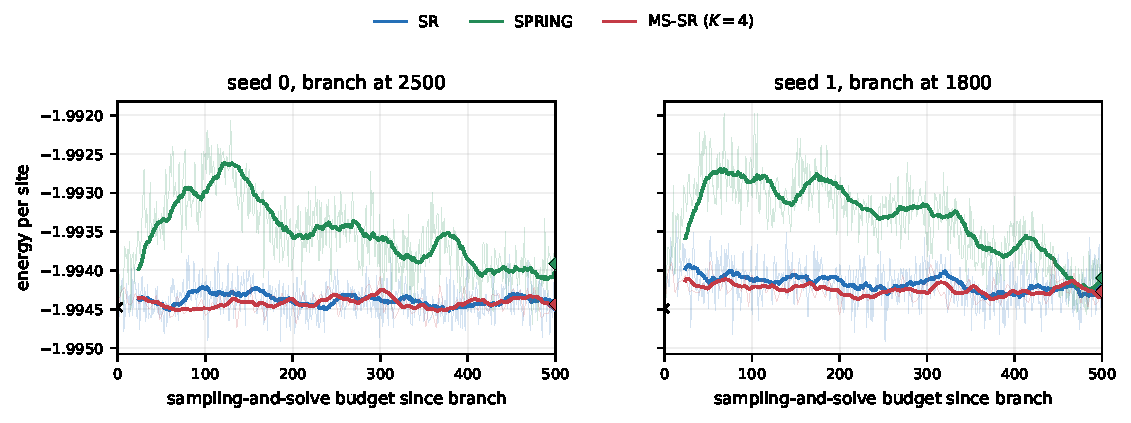
\includegraphics[width=\textwidth]{figures/figure5_equal_budget_online.pdf}
    \caption{Equal-budget late-stage online comparison on the $8\times8$
    $J_1$-$J_2$ model with a no-symmetry ViT. Each panel branches SR, SPRING,
    and fixed-grid MS-SR from identical parameters. One SR or SPRING update is
    one budget unit; one $K=4$ MS-SR update is four. Faint lines are raw
    training-energy estimates and solid lines are rolling means over a common
    25-budget-unit window. Diamonds are audited fresh-chain
    endpoint evaluations; bars are one conservative reported Monte Carlo
    standard error, not variation across seeds.}
    \label{fig:mssr_equal_budget_online}
\end{figure}

Figure~\ref{fig:mssr_equal_budget_online} compares two controlled late-stage
branches at equal sampling-and-solve budget. Each arm receives $500$ units, so
SR and SPRING take $500$ updates while MS-SR takes $125$.
For seed 0 (branch step 2500), MS-SR $-1.9944365\mathbin{\pm}7.06\times10^{-6}$, SR $-1.9944498\mathbin{\pm}6.86\times10^{-6}$, SPRING $-1.9939130\mathbin{\pm}8.36\times10^{-6}$. The numerical endpoint ordering (lower is better) is SR $<$ MS-SR $<$ SPRING; MS-SR minus SR is $+0.0000133$ per site ($+1.36$ combined endpoint Monte Carlo standard errors); MS-SR minus SPRING is $-0.0005235$ per site ($-47.84$ combined endpoint Monte Carlo standard errors).
For seed 1 (branch step 1800), MS-SR $-1.9942723\mathbin{\pm}7.83\times10^{-6}$, SR $-1.9942534\mathbin{\pm}7.88\times10^{-6}$, SPRING $-1.9940982\mathbin{\pm}8.02\times10^{-6}$. The numerical endpoint ordering (lower is better) is MS-SR $<$ SR $<$ SPRING; MS-SR minus SR is $-0.0000189$ per site ($-1.70$ combined endpoint Monte Carlo standard errors); MS-SR minus SPRING is $-0.0001741$ per site ($-15.53$ combined endpoint Monte Carlo standard errors).
These are two individual branched trajectories; the endpoint uncertainties
measure Monte Carlo evaluation error and do not estimate across-seed variation.
